\documentclass{scrartcl}
\usepackage{sagetex}
\usepackage[usenames,dvipsnames]{xcolor}
\usepackage{tkz-fct}
\pagestyle{empty}

\begin{document}
\begin{sagesilent}
x=var('x')
t = var('t')
x_coords = [t for t in srange(-6,3,.01)]
y_coords = [(-t^2+t+2)*exp(t) for t in srange(-6,3,.01)]
output = ""
for i in range(0,len(x_coords)-1):
    if ((y_coords[i]>=-5 and y_coords[i]<=6) and (y_coords[i+1]>=-5 and y_coords[i+1]<=6)):
        output += r"\draw[red, thick] (%f cm ,%f cm)--(%f cm ,%f cm);"%(x_coords[i],y_coords[i],x_coords[i+1],y_coords[i+1])

u = var('u')
f = (-u^2+u+2)*exp(u)
m(u) = diff(f,u,1)
tan_line(u)=m(0)*u+2
x1_coords = [u for u in srange(-2.6,1.8,.01)]
y1_coords = [tan_line(u) for u in srange(-2.6,1.8,.01)]

output1=""
for i in range(0,len(x1_coords)-1):
    if ((y1_coords[i]>=-5 and y1_coords[i]<=6) and (y1_coords[i+1]>=-5 and y1_coords[i+1]<=6)):
        output1 += r"\draw[blue, thick] (%f cm ,%f cm)--(%f cm ,%f cm);"%(x1_coords[i],y1_coords[i],x1_coords[i+1],y1_coords[i+1])
\end{sagesilent}

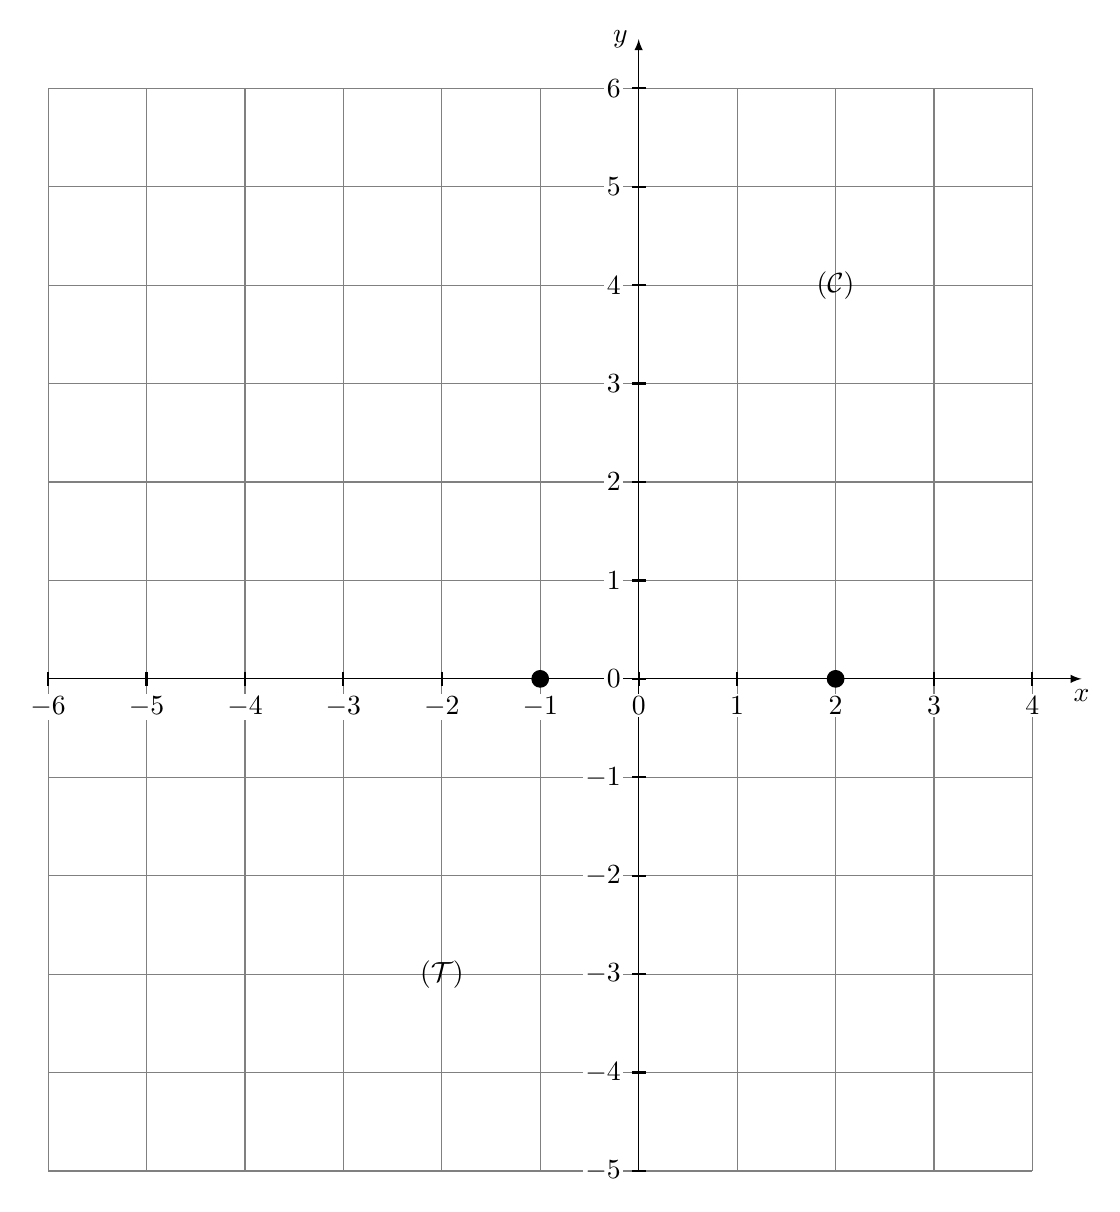
\begin{tikzpicture}[scale=1.25]
\tkzInit[xmin=-6,xmax=4,ymin=-5,ymax=6]
\tkzGrid
\tkzAxeXY
\sagestr{output}
\sagestr{output1}
\tkzSetUpPoint[size=6]
\tkzDefPoint(2,0){b} \tkzDrawPoint(b)
\tkzDefPoint(-1,0){c} \tkzDrawPoint(c)
\tkzText(2,4){($\mathcal{C}$)}
\tkzText(-2,-3){($\mathcal{T}$)}
\end{tikzpicture}
\end{document}
